\section{Concurrency}
\subsection{Motivation}
\subsubsection{Wieso wird Concurrency verwendet?}
\begin{itemize}
  \item Praktische Programme führen meist mehrere Arbeiten "`gleichzeitig"' aus. 
\end{itemize}
\subsubsection{Parallelität vs. Concurrent Computing}
\begin{itemize}
  \item Parallel Computing
  	\begin{itemize}
  	  \item execution of different tasks is really at the same time
  	  \item is not possible on a single-core machine 
  	\end{itemize}
  \item Concurrent Computing
  	\begin{itemize}
  	  \item execution of different tasks only seems to be at the same time
  	  \item different tasks get consecutive time slices
  	  \item there's only one task really running at a particular time slice
  	  \item can be done on a single- or multicore machine 
  	\end{itemize} 
\end{itemize}
\subsubsection{Gründe, Concurrency nicht zu verwenden}
\begin{itemize}
  \item Concurrency (mit Prozessen, Tasks, Threads) kostet immer
  \begin{itemize}
  	\item Stack
  	\item Context switch (Umschalten vom einen zum anderen) 
  	  \begin{itemize}
  	  \item dauert
  	  \item Alter Context muss gespeichert, neuer wieder geladen werden
  	  \end{itemize}
  	\item Zugriff auf gemeinsame Ressourcen muss synchronisiert werden 
  	  \begin{itemize}
  	  \item kostet
  	  \item fehleranfällig (wird vergessen oder falsch gemacht)
  	  \end{itemize}
  \end{itemize}
\item Komplexität steigt
  \begin{itemize}
  \item Sequentielle Programme sind einfacher zu verstehen als parallele
  \item Ziel ist immer, ein System möglichst einfach zu halten
  \end{itemize}
\end{itemize}

\textbf{Folgerung:} Concurrency nur dann einsetzen, wenn wirklich ein Nutzen vorhanden ist!

\subsection{POSIX Threads Programming}
\subsubsection{UNIX Process}
\begin{itemize}
\item Heavyweight process (created by the operating system)
\item Processes require a fair amount of overhead; they contain information about program resources and program execution state, including: Process ID, process group ID, user ID, and group ID; Enviroment; Program instructions; Registers; Stack; Heap; File descriptors; Signal actions; Shared libraries; Inter-process communication tools
\end{itemize}
\subsubsection{UNIX Thread}
\begin{itemize}
\item Lightweight "process"
\item Threads use and exist within the process resources
\item A thread uses the same address space as other threads of the same process
\item Threads are able to be scheduled by the operating system
\item Independent stream of instructions that may run simultaneously to other streams of instructions
\item Procedure that runs independently from its main program
\item A thread maintains its own: Stack pointer; Registers; Scheduling properties; Set of pending and blocked signals; Thread specific data
\item Concurrent programs are usually achieved with threads
\end{itemize}
\subsubsection{Process vs. Thread in UNIX}
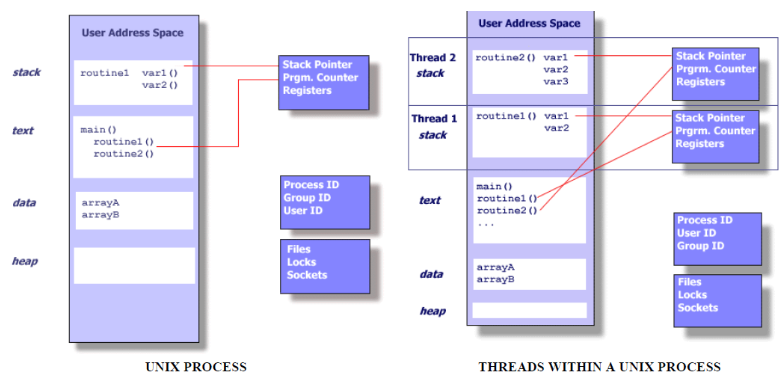
\includegraphics[width=12cm]{images/Concurrency/ProcessVsThread.png}\\\\
Man beachte: Alles was ein Thread inne hat, hat ein Prozess auch inne (aber NICHT umgekehrt)!
\subsubsection{What are POSIX Threads?}
\begin{itemize}
\item For UNIX systems, a standardized C language threads programming interface has been specified by the IEEE POSIX 1003.1c standard.
\item The short form of POSIX threads is Pthreads or pthreads.
\end{itemize}
\subsubsection{The pthreads API}
\begin{itemize}
\item Routines of the pthreads API start with pthread\_
\item The header file pthread.h must be included
\item The link command must include –lpthread
\end{itemize}
\subsubsection{Starting and Terminating a Thread}





Quasiparallelität:\\
Prozesse/Threads können folgende Zustände und Übergänge erfahren: 
\begin{center}
{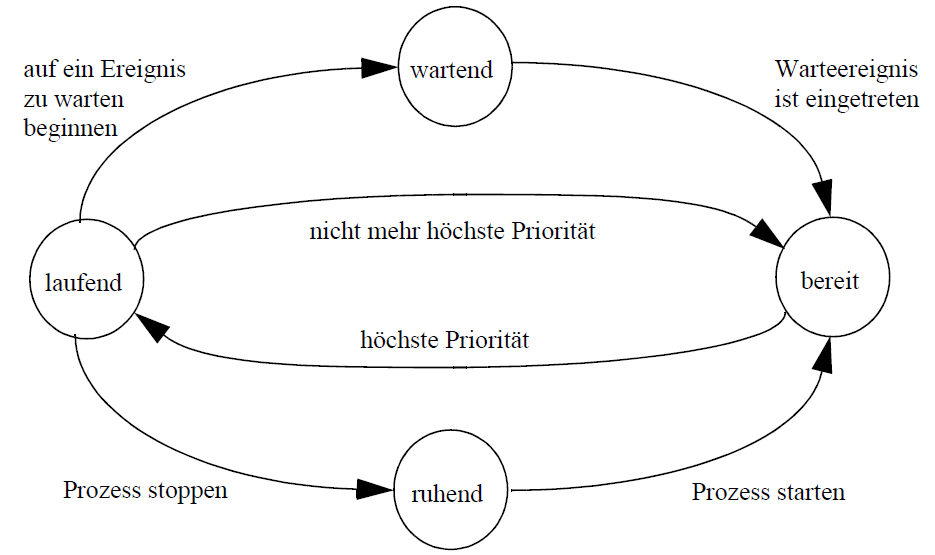
\includegraphics[width=0.5\textwidth]{images/Concurrency/Prozesszustaende.png}}
%\label{Fig: Schlechtes Beispiel für Modularisierung}
\end{center}

\begin{itemize}
  \item Threads aus Standardklasse System.Threading
  \item Jede \textbf{parameterlose void-Methode M} kann zu einem Thread gemacht
  werden 
\end{itemize}
\begin{centering}
  \begin{lstlisting}[style=C]
  Thread t = new Thread(new Threadstart(M));
  \end{lstlisting}
\end{centering}
\begin{itemize}
  \item Dem Thread-Ctor muss das Delegate \textbf{ThreadStart} übergeben werden
  \item Der Thread wird gestartet mit:  
\end{itemize}
\begin{centering}
  \begin{lstlisting}[style=C]
  t.Start();
  \end{lstlisting}
\end{centering}
\begin{itemize}
  \item Beenden des Threads: 
  \begin{itemize}
    \item Ende seiner Methode
    \item Explizierter Abrruch mitttels Abort()  
  \end{itemize} 
\end{itemize}
\begin{center}
{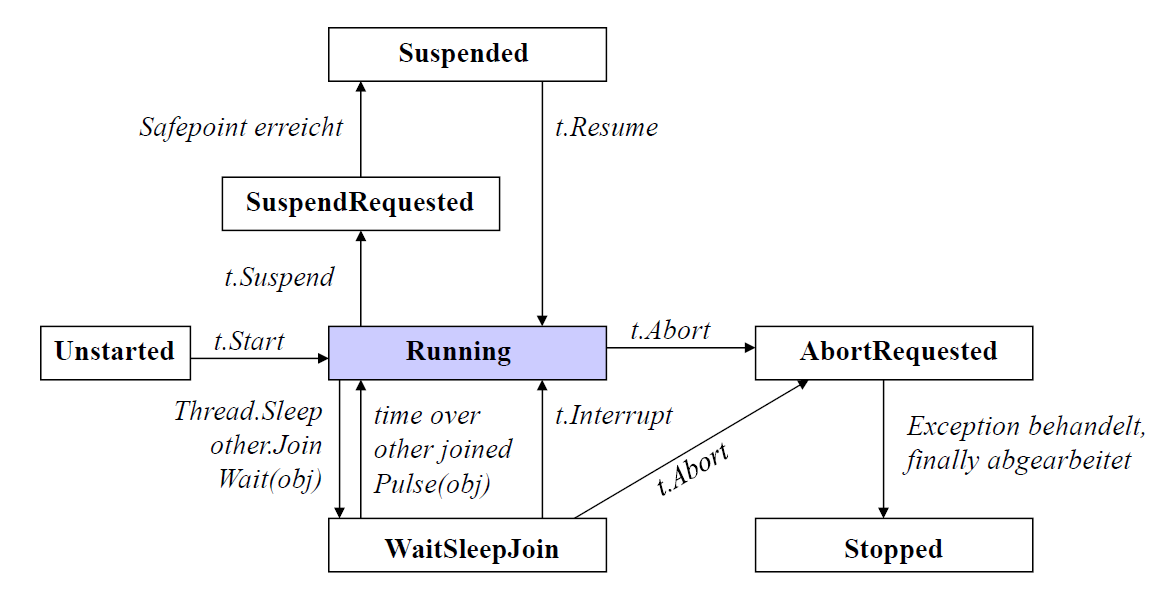
\includegraphics[width=0.5\textwidth]{images/Concurrency/Zustandsuebergaenge.png}}
%\label{Fig: Zustandübergänge}
\end{center}

Thread-Zustände:
\begin{lstlisting}[style=CSharp]
Thread t = new Thread(P);
Console.WriteLine("name={0}, priority={1}, state={2}", t.Name, t.Priority, t.ThreadState);
t.Name = "Worker"; t.Priority = ThreadPriority.BelowNormal;
t.Start();
Thread.Sleep(1);
Console.WriteLine("name={0}, priority={1}, state={2}", t.Name, t.Priority, t.ThreadState);
t.Suspend();
Thread.Sleep(1);
Console.WriteLine("state={0}", t.ThreadState);
t.Resume();
Console.WriteLine("state={0}", t.ThreadState);
t.Abort();
Thread.Sleep(1);
Console.WriteLine("state={0}", t.ThreadState);
\end{lstlisting}



\subsection{Beispiele}
Allgemeines Beispiel:
\begin{lstlisting}[style=C]
  //Zwei Programme, die staendig Zeichen auf dem Bildschirm ausgeben
  using System; 
  usign System.Threading; 
  class Printer
  {
    char ch; 
    int sleepTime; 
    public Printer(char c, int t)
    {
      ch = c;
      sleepTime = t; 
    }
    public void Print()
    {
      for(int i=0; i<100; i++)
      {
        Console.Write(ch); 
        Thread.Sleep(sleepTime); 
      }
    }
  }
  class Test
  {
    static void Main()
    {
      Printer a = new Printer('.',10);
      Printer b = new Printer('*',100);
      new Thread(a.Print).Start(); 
      new Thread(b.Print).Start();   
    }
  }
  //Das Programm laeuft so lange, bis der letzte Foreground-Thread beendet ist.
\end{lstlisting}

Beispiel für Join:
\begin{lstlisting}[style=C]
  using System; 
  usign System.Threading; 
  class Test
  {
    static void P()
    {
      for(int i=0; i<20; i++)
      {
        console.Wirte('-');
        Thread.Sleep(100);  
      }
    }
  }

  static void Main()
  {
    Thread t = new Thread(P); 
    Console.Write("start"); 
    t.Start(); 
    t.Join(); //Wartet auf t
    Console.WriteLine("end");   
  }
  //Ausgabe: start--------------------end
\end{lstlisting}
  
Threads abbrechen:
\begin{itemize}
  \item Automatisches abbrechen, sobald der Worker-Thread das Ende seiner Methode
  erreicht hat. 
  \item Ein Thread kann explizit mit Abort() abgebrochen werden
  $\rightarrow$ Dabei wird eine ThreadAbortException ausgelöst, die in der
  Thread-Methode abgefangen und behandelt werden muss. 
\end{itemize}
\begin{lstlisting}[style=C]
    using System;
    using System.Threading; 
    class Test
    {
      static void P()
      {
        try
        {
          try
          {
            try
            {
              wile(true); 
            }
            catch(ThreadAbortException)
            {
              Console.WriteLine("-- inner aborted"); 
            }
          }
          catch(ThreadAbortException)
          {
            Console.WriteLine("-- outer aborted"); 
          }
        }
        finally
        {
          Console.WriteLine("-- finally"); 
        }
      }
      
      static void Main(string[] arg)
      {
        Thread t = new Thread(P); 
        t.Start(); 
        Thread.Sleep(1); 
        t.Abort(); 
        t.Join(); 
        Console.WriteLine("done"); 
      }
    }
    //Ausgabe: 
    //-- inner aborted
    //-- outer aborted
    //-- finally
    //done
\end{lstlisting}

\subsection{Synchonisation: Zugriff auf gemeinsame Ressourcen \buch{p.21}}
Definition kritischer Bereich: 
\begin{itemize}
  \item Codebereich, in dem nebenläufige Prozesse auf gemeinsame Ressource
  zugreifen. 
  \item Zu jeder Zeit darf sich höchstens ein Prozess im kritischen Bereich
  aufhalten. 
  \item Dies wird mittels gegenseitigem Ausschluss (Mutual Exclusion, Mutex)
  sicher gestellt. 
\end{itemize}
Forderungen an die Synchronisation (Dijkstra, 1965)
\begin{itemize}
  \item Zwei Prozesse dürfen sich nicht gleichzeitig in einem kritischen Bereich
  befinden (Mutex).
  \item Über Abarbeitungsgeschwindigkeit und Anzahl Prozesse dürfen keine
  Annahmen getroffen werden. 
  \item Kein Prozess darf ausserhalb des kritischen Bereichs einen anderen
  Prozess blockieren. 
  \item Jeder Prozess, der auf den kritischen Bereich wartet, muss irgendwann
  den Abschnitt betreten dürfen (fairness condition). 
\end{itemize}


\begin{tabbing}
  \hspace*{1cm}\=\hspace*{4.2cm}\=\hspace*{3cm}\=\hspace*{2.7cm}\= \kill
  Synchro-Versuch 1\\
  \>{\bf Prozess 1} \> \> \>{\bf Prozess 2}\\
  \>\begin{lstlisting}[style=C]
      while(grant != 1)
        wait(); 
      CS; //Eintritt in Critical Section 
      grant = 2; 
    \end{lstlisting} \> \> \>
    \begin{lstlisting}[style=C]
      while(grant != 2)
        wait(); 
      CS; //Eintritt in Critical Section  
      grant = 1; 
    \end{lstlisting} \\
    Forderung 2 nicht erfüllt, da sich alle Prozesse selbst daran hindern 2mal nacheinander daran zu kommen.\\\\
    
  Synchro-Versuch 2\\
   \>{\bf Prozess 1} \> \> \>{\bf Prozess 2}\\
   \>\begin{lstlisting}[style=C]
      while(in2)
        wait(); 
      in1 = true; 
      CS; //Eintritt in Critical Section 
      in1 = false; 
    \end{lstlisting} \> \> \>
    \begin{lstlisting}[style=C]
      while(in1)
        wait(); 
      in2 = true; 
      CS; //Eintritt in Critical Section 
      in2 = false; 
    \end{lstlisting} \\
    Initialisierung ist nicht gelöst.\\\\
\end{tabbing}
\newpage
\begin{tabbing}
  \hspace*{1cm}\=\hspace*{4.2cm}\=\hspace*{3cm}\=\hspace*{2.7cm}\= \kill
  Synchro-Versuch 3\\
   \>{\bf Prozess 1} \> \> \>{\bf Prozess 2}\\
   \>\begin{lstlisting}[style=C]
        request1 = true; 
        grant = 1; 
        while(grant==1 && request2)
          wait(); 
        CS; //Eintritt in Critical Section  
        request1 = false; 
    \end{lstlisting} \> \> \>
    \begin{lstlisting}[style=C]
        request2 = true; 
        grant = 2; 
        while(grant==2 && request1)
          wait(); 
        CS;  //Eintritt in Critical Section 
        request2 = false;  
    \end{lstlisting} \\ 
\end{tabbing}

Signale:
\begin{itemize}
  \item Jeder Prozess wartet vor Betreten des kritischen Bereihs auf ein
  gemeinsames Signal. 
  \item Wenn Signal gesetzt $\rightarrow$ kritischer Bereich frei
  \item waitfor(signal) blockiert aufrufenden Prozess, falls signal nicht
  gesetzt
  \item Jeder Prozess, der fertig ist, setzt Signal mit send(signal)
  \item Mehrere Prozesse können gleichzeitig warten 
\end{itemize}

\begin{tabbing}
  \hspace*{1cm}\=\hspace*{4.2cm}\=\hspace*{3cm}\=\hspace*{2.7cm}\= \kill
  Synchronisation mit Signalen\\
  \>{\bf Prozess 1} \> \> \>{\bf Prozess 2}\\
  \>\begin{lstlisting}[style=C]
      waitFor(signal); 
      CS;  //Eintritt in Critical Section 
      send(signal); 
    \end{lstlisting} \> \> \>
    \begin{lstlisting}[style=C]
      waitFor(signal); 
      CS;  //Eintritt in Critical Section 
      send(signal); 
    \end{lstlisting} \\\\
 \end{tabbing}
 
 \subsection{Semaphoren \buch{p.31}}
 \begin{itemize}
   \item Das Signal für den Zutritt in den kritischen Bereich = Semaphor
   \item Ein Semaphor s hat zwei atomare (= nicht unterbrechbare)
     Operationen
   \begin{itemize}
     \item P(s) : Passieren $\rightarrow$ Beim Eintritt in CS (waitFor)
     \item V(s) : Verlassen $\rightarrow$ Beim Austritt aus CS (send)
   \end{itemize}
   \item Probleme bei Semaphoren
   \begin{itemize}
    \item Anwendung erfordert Disziplin
    \begin{itemize}
      \item Jedes P(s) braucht ein V(s)
      \item Probleme treten auf, wenn V(s) vergessen geht!
      \item Beim Auftreten einer Exception kann das Freigeben ebenfalls
      schwierig sein. 
    \end{itemize}
   \end{itemize}
 \end{itemize}
 

 \subsection{Das Monitorprinzip \buch{p.35}}
 \begin{itemize}
   \item Grundprinzip: Abstrakten Datenyp definieren, der genau die Funktionen
   in der Schnittstelle anbietet, die notwendig sind. 
   \item Der Aufrufer ruft diese Funktionen auf, er muss sich aber nicht um die
   Synchro kümmern. 
   \item Die Synchro (z.Bsp. mit Semaphoren) ist in der Implementation des
   Monitors lokal gelöst. 
   \item Problem wird einmal im Monitor gelöst, die Aufrufer müssen sich nicht
   mehr darum kümmern. 
 \end{itemize}

\newpage
 \subsection{Thread-Synchronisation in CSharp \buch{p.36}} 
Beispiel Mutual Exclusion 
\begin{multicols}{2}
\begin{lstlisting}[style=C]
  //lock(Variable) Statement
  class Account
  {
    long val = 0; 
    public void Deposit(long x)
    {
      lock(this){val += x;} //jeweils nur 1 Thread darf diese Anweisung ausfuehren.
    }
    public void Withdraw(long x)
    {
      lock(this){val -= x; }
    }
  }
\end{lstlisting} 

\columnbreak

\textit{lock(this)} innerhalb eines Thread gilt nur den eigenen Thread, für andere Threads gilt dies nicht mehr.

\end{multicols}

Lock lässt sich auf beliebiges anderes Objekt setzen
\begin{multicols}{2}

\begin{lstlisting}[style=C]
  object semaphore = new object(); 
  ...
  lock (semaphore){..critical section...}
\end{lstlisting} 
\columnbreak

Die Anweisung \textit{lock} geht nur wenn es von System.Object erbt. z.B ein int kann nicht gelockt werden.
Eine Semaphore muss \textit{static} und ein \textit{Object} sein.

\end{multicols}

Klasse Monitor:\\
\begin{lstlisting}[style=C]
  lock(v) 
  ... ist Kurzform fuer ...
  try
  {
    Statement
  }
  finally
  {
    Monitor.Exit(v); 
  }
\end{lstlisting} 
Wenn Thread während der Ausführung von Statement mit Abort abgebrochen wird,
wird trotzdem finally ausgeführt und der monitor frei gegeben.\\

Wait und Pulse:
\begin{tabbing}
  \hspace*{1cm}\=\hspace*{4.2cm}\=\hspace*{3cm}\=\hspace*{2.7cm}\= \kill
  Beispiel:\\
  \>{\bf Thread A} \> \> \>{\bf Thread B}\\
  \>\begin{lstlisting}[style=C]
      lock(v) //1
      {
       ...
       Monitor.Wait(v); //2
       ...
      }
    \end{lstlisting} \> \> \>
    \begin{lstlisting}[style=C]
      lock(v) //3
      {
        ...
        Monitor.Pulse(v); //4
        ...
      }//6
    \end{lstlisting} \\\\
\end{tabbing}
\begin{enumerate}
   \item A kommt zu lock(v) und erhält Eintritt, da kein anderer Thread im
   gesperrten Bereich ist. 
   \item A kommt zu Wait, legt sich schlafen und gibt die Sperre frei. 
   \item B kommt zu lock(v) und erhält Eintritt, da die Sperre frei ist. 
   \item B kommt zu Pulse und weckt damit A. Es kann (aber muss nicht) ein
   Thread-Wechsel statt finden. 
   \item A versucht, die Sperre wieder zu erlangen, was aber nicht gelingt, da B
   sie noch hat. 
   \item B gibt am Ende des gesperrten Bereichs die Sperre frei, A kann nun
   wieder eintreten und weiter laufen. 
\end{enumerate}
Beachte: 
\begin{itemize}
   \item Wait(v) und Pulse(v) dürfen nur in einer Anweisungsfolge aufgerufen
   werden, die mit lock(v) geschützt wurde.
   \item Zwischen Pulse(v) und dem dadurch geweckten Thread können andere
   Threads zur Ausfürhung gelangen, die in der Zwischenzeit versucht haben, die
   Sperre zu bekommen\\ $\rightarrow$ Die Bedingung von Pulse muss nach wait
   nicht mehr gelten!\\
   Daher sollte man die Wait-Bedingung immer in einer Schleife prüfen: 
\end{itemize}
\begin{lstlisting}[style=C]
  while(condition false)
    Monitor.Wait(v); 
  ...
  make condition true;
  Monitor.Pulse(v);       
\end{lstlisting}
\begin{itemize}
  \item PulseAll(v) weckt alle in v wartenden Threads, aber nur einer darf in
  den gesperrten Bereich. Der nächste darf erst rein, wenn der Vorgänger die
  Sperre frei gibt.
\end{itemize}

\subsubsection{Beispiel: Bufferverwaltung}
\begin{multicols}{2}
\begin{lstlisting}[style=C]
  class Buffer
  {
    const int size = 4; 
    char[] buf = new char[size];
    int head = 0; 
    int tail = 0; 
    int n = 0; 
    
    public void Put(char ch)
    {
      lock(this)
      {
        while(n==size)
          Monitor.Wait(this); 
        buf[tail] = ch; 
        tail = (tail+1)%size; 
        n++; 
        Monitor.PulseAll(this); 
      }
    }
    
    public char Get()
    {
      lock(this)
      {
        while(n==0)
          Monitor.Wait(this); 
        char ch = buf[head]; 
        head = (head+1)%size; 
        n--; 
        Monitor.PulseAll(this); 
        return ch; 
      }    
    }
  }      
\end{lstlisting}

\columnbreak

Ablauf, wenn Producer schneller:\\
Put\\
Put\\
Put\\
Put\\
Get\\
Put\\
Get\\
\ldots

Ablauf, wenn Consumer schneller:\\
Put\\
Get\\ 
Put\\
Get\\
\ldots

\end{multicols}

\subsection{Petri-Netze \buch{p.42}}
\subsubsection{Elemente \buch{p.45}}
  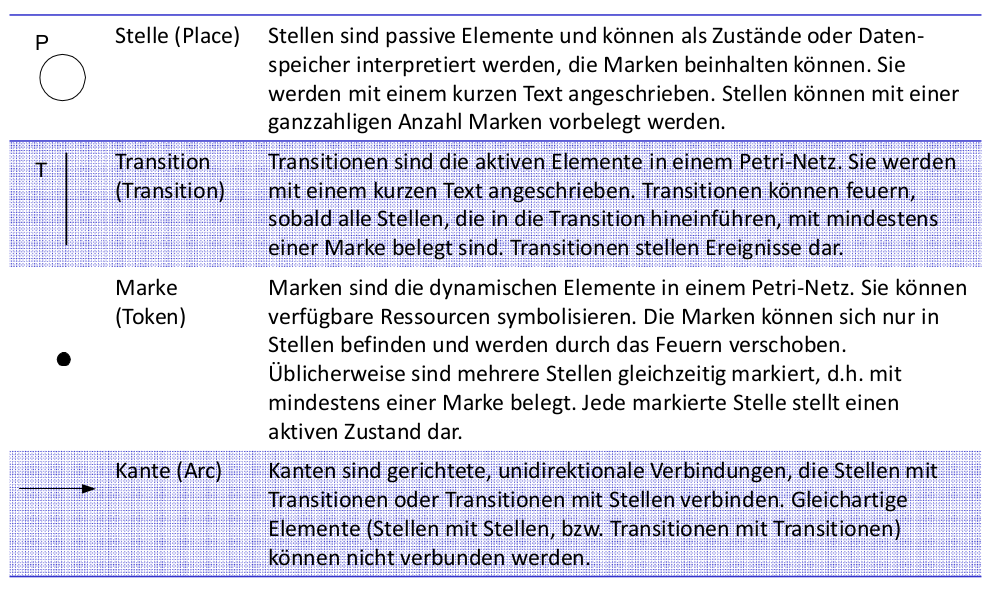
\includegraphics[width=15cm]{images/Concurrency/PetriNetzeElemente}
  
\subsubsection{Feuern von Transitionen \buch{p.46}}
  Eine Transistion kann nur dann feuern, wenn alle Stellen, die in die Transition hineinführen mit min.
  1 Marke belegt sind. Bei den Eingabestellen wird dann 1 Marke entzogen und bei den Ausgabestellen eine hinzugefügt.

\begin{description}
  \item[Race Condition]  Das Ergebnis einer Operation hängt von zeitlichen Verhalten bestimmter Einzeloperationen ab.
  \item[Starvation]      Ist ein Zustand, bei dem ein Prozess nie dran kommt (er verhungert). 
  \item[Deadlock]        Ist eine Situation in denen sich zwei Prozesse gegenseitig blockieren.
\end{description}


